%
% File ccl2024-zh.tex
%
%%
%% Based on the original version of COLING-2018 file (coling2018.tex), with changes made by Yue Zhang.
%%

\documentclass[11pt]{article}
\usepackage[utf8]{inputenc}
\usepackage[hyperref]{ccl2024-zh}
\usepackage{url}

\usepackage[ruled,linesnumbered]{algorithm2e}

\usepackage{latexsym}
\usepackage{CJKutf8}

\usepackage{indentfirst}
\usepackage{fancyhdr}
\usepackage{graphicx}
\usepackage{tabularx}
\usepackage{multirow}

\pagestyle{fancy}
\fancyhf{}
\lhead{\begin{CJK*}{UTF8}{gbsn}计算语言学\end{CJK*}}
\renewcommand{\headrulewidth}{0pt}

% \setlength\titlebox{5cm}

% You can expand the titlebox if you need extra space
% to show all the authors. Please do not make the titlebox
% smaller than 5cm (the original size); we will check this
% in the camera-ready version and ask you to change it back.



\title{面向CQL的语料库检索引擎的高效实现}
\englishtitle{Efficient implementation of a CQL-oriented corpus retrieval engine}

\date{}


\begin{document}
\begin{CJK*}{UTF8}{gbsn}
\setlength{\parindent}{2em}

% Make Chinese title and abstract
\maketitle
\begin{abstract}
  
%本文提出了一种面向CQL的高效语料库检索引擎实现方法。首先,利用ANTLR工具对CQL语句进行语法分析,将得到的语法树转换为语料库检索式。其次,在构建语料数据库时,我们采用了优化的倒排索引表,实现了对非词表词语的快速检索。然后,在检索过程中,我们采取了两阶段策略:第一阶段忽略位置和距离约束,进行初步检索,并通过候选标记位方法迅速合并多个检索单元的候选列表;第二阶段则对候选列表应用约束条件进行二次匹配和过滤。最终,生成精确的候选语料列表。实验证明,该检索引擎在《人民日报》图文数据库上展现了高效且准确的性能,为语料库检索领域提供了新的解决方案和工程实践经验。
语料库检索引擎在语言学研究中扮演着核心角色,对于高效获取信息至关重要。然而,当前国内语料库检索引擎在检索语言上缺乏统一标准,尤其支持CQL的中文语料库检索工具相对稀缺。在使用BlackLab进行中文语料库检索时,我们遇到了由于分词工具切分粒度问题导致的数据召回难题。为应对这些挑战,我们研发了一款支持CQL语言检索且兼容多粒度分词的语料库检索引擎。经过多种分词器的测试,该引擎展现出了优异的召回率,并在性能上达到了甚至超越了BlackLab的检索速度,为语言学工作者提供了更加高效、精准的检索工具。


  \keywords{语料库查询语言 \and 语料库检索 \and 倒排索引}
\end{abstract}

% Make English title and abstract
\makeenglishtitle
\begin{englishabstract}
	
This paper proposes an efficient implementation method for a CQL-oriented corpus retrieval engine. Firstly, the ANTLR tool is utilized to perform syntactic analysis on CQL statements, converting the resulting syntax tree into a corpus retrieval expression. Secondly, when constructing the corpus database, we adopt an optimized inverted index table to enable rapid retrieval of non-lexical words. Then, during the retrieval process, we adopt a two-stage strategy: in the first stage, positional and distance constraints are ignored to perform preliminary retrieval, and the candidate lists of multiple retrieval units are quickly merged using the candidate marking method; in the second stage, constraint conditions are applied to the candidate lists for secondary matching and filtering. Finally, an accurate candidate corpus list is generated. Experiments demonstrate that this retrieval engine exhibits efficient and accurate performance on the People's Daily graphic database, providing a new solution and engineering practical experience for the field of corpus retrieval.

  
  \englishkeywords{corpus query language \and corpus retrieval \and  inverted index}
\end{englishabstract}

\section{引言}
\label{intro}

随着语言学的深入研究和信息技术的迅猛发展,语料库作为语言学研究的基础资源,其重要性日益凸显。语料库检索引擎作为从这一宝贵资源中获取信息的核心工具,对于高效、准确地挖掘语言数据具有关键作用。然而,当前国内语料库检索引擎在技术和应用层面仍存在诸多挑战。

首先,尽管市场上已有一些语料库检索系统,如北京大学的CCL现代汉语语料库\cite{ccl}和北京语言大学的BCC语料库\cite{bcc},它们拥有丰富的语料资源和多样的功能,但各自使用的查询语言语法差异显著。这意味着用户在使用不同的语料库时,需要学习并掌握各自独特的检索语法和规则,这无疑增加了用户的学习成本和使用难度。

其次,在语料库检索领域,尽管检索表达式的多样性和复杂性体现了其强大的功能,但同时也导致了非标准化的问题。不同的语料库系统采用不同的检索语法,使得用户在使用不同系统时需要适应不同的检索方式。这种现状不仅影响了用户的使用体验,也制约了语料库检索工具的进一步普及和应用。

此外,随着语料库查询语言(Corpus Query Language 简称,CQL)的广泛应用,越来越多的语料库检索工具开始采用这一标准。CQL以其简洁直观的语法、灵活多样的检索方式以及强大的扩展性,赢得了语言学家的青睐。然而,在中文语料库检索中,由于中文词语的边界模糊和分词的不确定性,使得CQL的应用面临诸多挑战。

特别是在使用基于Lucene引擎的检索工具如BlackLab时,中文分词的问题尤为突出。由于中文词语的切分粒度不固定且存在一定的歧义性,用户在检索时往往难以确定哪些词语可以作为有效的检索词。这不仅影响了检索的准确性和效率,也制约了BlackLab等语料库检索工具在中文语料库研究中的进一步应用。

针对上述问题,我们研发了一款支持CQL语言检索且兼容多粒度分词的语料库检索引擎。该引擎通过优化索引结构、改进检索算法以及支持多种分词粒度查询等方式,有效解决了中文分词带来的检索难题。经过多种分词器的测试验证,该引擎展现出了优异的召回率和检索速度,为语言学工作者提供了更加高效、精准的检索工具。这一创新性的研发成果不仅推动了计算语言学研究的发展,也为中文语料库检索技术的进步做出了贡献。

%https://stanfordnlp.github.io/CoreNLP/index.html
%
%语料库作为自然语言处理研究的基础资源,其重要性日益凸显。语料库检索引擎作为从语料库中获取信息的核心工具,其性能和效率直接影响到研究者的工作效率和成果质量。因此,构建一个高效、灵活的语料库检索引擎对于推动计算语言学研究具有重要意义。
%
%目前,尽管已有一些语料库检索系统,例如:北京大学CCL现代汉语语料库\cite{ccl}、北京语言大学BCC语料库等中文语料库\cite{bcc},拥有庞大的语料资源,提供了丰富的功能,但这些语料库分析工具使用的查询语言的语法差异较大\cite{zhangyongwei}。这意味着用户在使用这些语料库时,需要分别学习和掌握各自的检索语法和规则。语料库检索的复杂性和多样性主要体现在其检索表达式的非标准化上。不同的语料库系统通常采用不同的检索语法,这导致了用户在使用不同系统时需要学习和适应不同的检索方式,增加了使用难度和成本。
%
%
%在本研究中,我们将重点探讨语料库检索引擎的实现,探讨如何使用更为通用的语料库检索语言进行语料库查询,以及如何建立语料数据库,优化索引结构的改进检索算法等。我们希望通过这些努力,为用户提供一个更加快速、准确、灵活的语料库检索工具,从而推动计算语言学研究的进一步发展。

%
% The following footnote without marker is needed for the camera-ready
% version of the paper.
% Comment out the instructions (first text) and uncomment the 8 lines
% under "final paper".
%
\cclfootnote{
    %
    % for review submission
    %
    \hspace{-0.65cm}  % space normally used by the marker
    % 最终版论文请将许可声明放在此处。请参阅说明中的~\ref{licence}部分来准备论文。
    \textcopyright 2024 中国计算语言学大会

    \noindent 根据《Creative Commons Attribution 4.0 International License》许可出版
}

\section{背景}
\label{backgound}

随着信息技术的蓬勃发展,语料库查询语言逐渐走向通用化,语料库检索工具也日趋成熟和完善。在这一背景下,BlackLab\footnote[1]{https://github.com/INL/BlackLab}作为一款基于Lucene\footnote[2]{https://lucene.apache.org}引擎的检索工具,以其出色的性能和广泛的应用,为语言学家提供了强有力的支持。然而,不容忽视的是,由于中文词语边界的模糊性和不确定性,使得在中文语料库上运用BlackLab进行检索时,用户面临着选择有效检索词的难题。这一问题不仅影响了检索的准确性和效率,也制约了BlackLab在中文语料库研究中的进一步应用。因此,如何克服中文词语边界的不确定性,提高中文语料库检索性能,成为当前亟待解决的重要问题。

\subsection{语料库查询语言}

语料库作为语言学研究的重要工具,其查询语言也经历了不断的演变与完善。其中,语料库查询语言是从语料库查询处理器(Corpus Query Processor,简称CQP)发展而来的一系列语言,提供了词汇、短语和语法等语言学层面丰富检索功能\cite{wuliangping},逐渐成为语料库检索领域的主流语言。语料库查询语言(Corpus Query Lingua Franca,简称CQLF)已经成为国际标准ISO 24631-1 \cite{banski-etal-2016-corpus},在国际范围内的广泛认可与应用。

目前,众多语料库检索工具均采用了CQL作为检索语言,如CQPweb\cite{hardie2012cqpweb}、Sketch Engine\cite{sketchengine1}、BlackLab\cite{blacklab}等。CQL为这些工具带来高效、便捷的语料库检索体验,CQL语句按照功能可以分为简单检索、检索条件、检索范围\cite{Lu2024FromTT}:

(1)检索单元:检索单元是对一个词语的属性进行检索,通过编写具体的检索表达式产生具体的查询结果。检索单元可以一次检索一个属性,比如词语的词形或者词性等,如[word=“学习”]或者[pos!=“NR”],还可以使用布尔运算符连接多个表达式,实现对多个属性的检索。如[word=“学习” \& pos=“VV”]表示查询包含“学习”作为动词的语料。检索式的属性值,除了具体属性值以外,还支持使用正则表达式进行词语的模糊查询。多个检索单元的横向叠加就可以是实现对多个词语属性的检索。在语料匹配时,检索系统会对CQL语句从左到右进行检索单元的匹配,可处理连续型短语、非连续型短语以及非连续且位置变异型短语\cite{wuliangping}。

(2)检索范围,CQL可以使用within操作符,限定检索范围。范围约束标签可以是特定范围内的单词,比如\textless s\textgreater 表示以句子为匹配范围进行搜索,还可以和其它查询一起使用。

(3)约束条件,CQL还支持限定标签的使用,用户可以为检索单元赋予标签名,然后通过"::"后面的限定条件,指定标签之间的逻辑关系,实现单词检索单元之间的条件约束。例如,在CQL语句:“A:[]B:[] :: A.pos = B.pos”中,为检索单元定义了标签,A、B,指定的约束条件是A、B两个检索单元的词性必须相同。

CQL语言在语法上十分简洁直观,采用统一的约束符号,使得用户能够更快速地掌握语料库的使用方法。更为直接和自然的方式来表达检索需求,使得检索条件更加清晰明确,减少了歧义和误解的可能性。语法结构更加灵活,能够支持更复杂的检索需求。CQL语句示例如表\ref{cqltable}所示。

\begin{table}[h]
	\begin{center}
		\begin{tabular}{c|c|c}
			\hline \bf 功能 & \bf 示例 & \bf 说明 \\ \hline
			\multirow{4}{*}{检索单元}& [word=“学习”] & 包含“学习”的语料 \\ \cline{2-3} & [word=“编辑” \& pos=“VV”] & 包含"编辑"作为动词的语料 \\ \cline{2-3}
			& [word=“热爱”][word=“学习”] & “热爱”、“学习”连续出现的语料  \\ \cline{2-3} & [word='不但'][]\{0,5\}[word='而且'] & "不但"和"而且"间隔5字内的语料 \\ \hline
			检索范围 & [word='科技']within \textless s \textgreater & 在同一句中包含“科技”的语料 \\ \cline{1-3}
			约束条件 & A:[] [] B:[][] :: A.word = B.word & 包含形式如“有步骤有计划”语料 \\
			\hline
		\end{tabular}
	\end{center}
	\caption{\label{cqltable} CQL语句示例}
\end{table}


由于CQL在语法简洁性、直观性、灵活性以及扩展性等方面的优势,使用CQL作为语料库检索的主要语言。不仅能够降低学习成本,提高检索效率,还能够更好地满足用户的检索需求。

\subsection{倒排索引}

倒排索引\cite{Salton1974A}作为一种高效的信息检索手段,在现代信息处理和搜索引擎中发挥着关键作用。它的主要功能是记录词项在文档中的出现情况,建立词项反向映射到文档的索引关系,从而提高搜索效率和匹配度。

在语料库设计中,倒排索引的构建尤为重要。根据语料库系统采用的标签,如词语、词性等,系统需要建立这些标签与文档之间的倒排索引信息。这种索引关系使得语料库检索能够通过标签信息快速检索到包含这些标签的文档。倒排索引的优点在于其高效性和灵活性。通过预先建立索引,系统能够迅速处理大量查询请求,并支持复杂的查询操作和个性化的排序方式。此外,倒排索引还支持增量更新和扩展,以适应不断变化的文档集合和查询需求。

具体来说,倒排索引的构建过程包括分词、词性标注以及建立索引表等步骤。随后,系统根据这些信息建立一个倒排索引表,该表记录了词语与文档位置的映射关系。在检索过程中,用户输入的查询请求被系统解析为关键词,然后系统利用已建立的倒排索引查找这些关键词对应的文档位置信息。由于索引已经预先建立了关键词与文档之间的关联,系统能够迅速定位到相关文档并返回给用户。

倒排索引在全文搜索领域应用广泛,Lucene是全文搜索领域的杰出代表,它是一套用于全文检索的高性能、可伸缩的信息检索工具包。Lucene以其强大的文本分析、索引构建和查询处理能力,为开发者提供了灵活且高效的搜索解决方案。Lucene的核心在于其倒排索引技术,能够快速地定位到包含特定关键词的文档。通过分词、停用词过滤、词干提取等步骤,Lucene能够将原始文本转化为适合搜索的索引结构。Lucene在全文搜索领域有着举足轻重的地位,推动了信息检索技术的发展。

\subsection{BlackLab}

虽然Lucene检索功能十分强大,但语料库检索时,需要使用词语距离,词性约束、以及语法约束等复杂检索条件,因此Lucene无法直接用于语料库检索。BlackLab是基于Lucene引擎开发的一款专为语言学家设计,同时适用于历史研究和知识提取等领域的文本检索和分析工具。作为一款开源软件,BlackLab拥有强大的功能和灵活的使用方式。它能够索引标注文本,支持复杂模式的快速搜索,并可通过配置实现个性化索引。其强大的查询语言使得用户可以精确地定位所需信息,而灵活的搜索范围与结构设置则进一步增强了其适用性。此外,BlackLab还提供了丰富的结果处理功能,如匹配结果捕获、结果集分组与排序、高亮显示等,使得用户能够更高效地分析和利用搜索结果。

%在BlackLab检索中文语料库时,有一个突出的问题是用户无法确认那些词语可以用作检索词。其原因在于使用BlackLab建立中文语料库时,首先需要将语料数据进行分词,基于分词后的数据建立语料库。在语料库检索时,需要使用包含在分词词表中的词语进行检索,如果使用分词词之外的词语进行语料库检索,则无法获得结果。一方面中文词语数量众多,词语的切分单元并不固定,一些词语比如:“中华民族”,是应该被切分成“中华”、“民族”,还是应该作为一个完成词语,不同分词工具处理方式不同,用户很难知道这些词语在语料库中的切分粒度,另一方面中文分词本身就存在一定的歧义性,比如:“一个人”,是应该如何切分,还和语料上下文相关,不同的分词工具可能产生不同的分词结果。检索词的不确定性,这都给使用者带来不便。

在使用BlackLab进行中文语料库检索时,有一个突出的问题是用户难以确定哪些词语可以作为有效的检索词。这一问题的根源在于构建中文语料库时,需要对语料数据进行分词处理,而语料库的检索则必须依赖于分词词表中的词语。如果用户尝试使用分词词表之外的词语进行检索,将无法获得任何结果。

中文词汇的丰富性和切分单元的不确定性,使得这个问题尤为突出。\cite{zhangwenjing}指出不同的人工标注语料上,分词标准存在差异。以“在和平共处五项原则的基础上”这句为例,探讨了标注语料对“和平共处五项原则”这一段的切分存在较大差异,这也反映出在人的认知层面,中文词语的边界存在着模糊性。常用的中文分词工具也会因为训练语料与分词策列不同,对同一句子产生不同的分词结果。

本文选择常用的中文分词工具进行分词结果比较,可以看到分词一致性比较低,Stanford的分词工具\cite{corenlp}更倾向于切分出较小的单元,而结巴分词的分词粒度比较大,清华大学THULAC(THU Lexical Analyzer for Chinese)\cite{li-sun-2009-punctuation},哈尔滨工业大学的LPT(Language Technology Platform)\cite{che-etal-2021-n}的与中科院的大数据语义智能分析平台NLPIR\cite{zhanghuaping2019}的分词工具结果一致。

中文分词无论在工具层面还是在人的认知层面都存在差异,导致用户在语料库检索时,难以确定一段文字在语料库中的具体切分形式。这使得用户在选择检索词时\cite{ccl}感到困惑。

%Stanford [('在', 'P'), ('和平', 'AD'), ('共处', 'VV'), ('五', 'CD'), ('项', 'M'), ('原则', 'NN'), ('的', 'DEG'), ('基础', 'NN'), ('上', 'LC')]
%结巴 [('在', 'p'), ('和平共处', 'nz'), ('五项原则', 'n'), ('的', 'uj'), ('基础', 'n'), ('上', 'f')]
%中科院计算所 [('在', 'preposition'), ('和平共处', 'verb'), ('五', 'numeral'), ('项', 'classifier'), ('原则', 'noun'), ('的', 'particle'), ('基础', 'noun'), ('上', 'noun of locality')]
%清华大学 [('在', 'p'), ('和平共处', 'id'), ('五', 'm'), ('项', 'q'), ('原', 'a'), ('则', 'n'), ('的', 'u'), ('基础', 'n'), ('上', 'f')]
%哈尔滨工业大学 [('在', 'p'), ('和平共处', 'i'), ('五', 'm'), ('项', 'q'), ('原则', 'n'), ('的', 'u'), ('基础', 'n'), ('上', 'nd')]

\begin{table}[h]
	\begin{center}
		\begin{tabular}{c|c|c|c|c|c|c|c|c|c|c} \hline 
			\bf 分词工具 & \multicolumn{10}{c}{\bf 分词结果} \\ \hline
			Stanford & 在  & 和平  & 共处  & 五  & 项  & \multicolumn{2}{c|}{原则}  & 的  & 基础  & 上 \\ \hline
			Jieba & 在 & \multicolumn{2}{c|}{和平共处} & \multicolumn{4}{c|}{五项原则}  & 的  & 基础  & 上 \\ \hline
			LPT & 在 & \multicolumn{2}{c|}{和平共处} & 五 & 项 & \multicolumn{2}{c|}{原则} & 的 & 基础  & 上 \\ \hline
			NLPIR & 在 & \multicolumn{2}{c|}{和平共处} & 五 & 项 & \multicolumn{2}{c|}{原则} & 的 & 基础  & 上 \\ \hline
			THULAN & 在 & \multicolumn{2}{c|}{和平共处} & 五 & 项  & 原 & 则  & 的  & 基础  & 上 \\ \hline
		\end{tabular}
	\end{center}
	\caption{\label{ccl-table} 分词结果比较}
\end{table}

这种检索词的不确定性给使用者带来了极大的不便,不仅影响了检索的效率和准确性,还可能导致遗漏重要的信息。由于BlackLab严格以词语边界作为检索条件,因此在使用BlackLab进行中文语料库检索时,用户只有在选择与语料数据切分相一致的检索词的情况下,才可能获得正确的检索结果。

\section{我们的工作}

我们选择CQL语言作为语料库检索语言。采用C++语言开发了一款高效的语料库检索引擎,采用ANTLR工具进行CQL语句的解析,确保了语法解析的准确性和高效性。同时,我们改进倒排索引策略,解决非词典词语的匹配问题,并进行存储结构设计以及性能优化,采用两阶段检索策略,有效提升了检索速度,语料库检索流程如图\ref{fig:liucheng}所示。

\begin{figure}[!h]
	\centering
	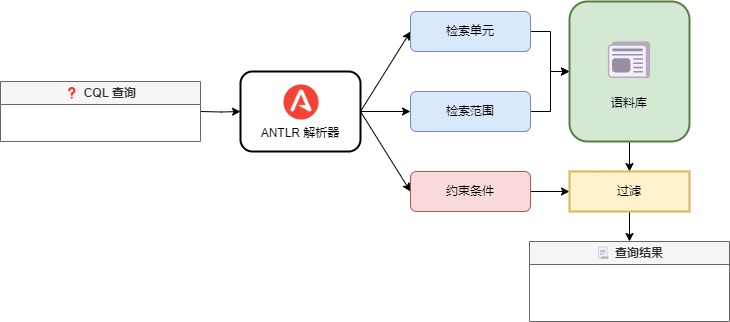
\includegraphics[width=0.7\textwidth]{image/liuchengtu.jpg}
	\caption{语料库检索流程图}
	\label{fig:liucheng}
\end{figure}

\subsection{CQL语法解析}

CQL具有良好的人类可读性,但如果使用CQL实现语料库的检索,还需要将其转换为计算机可执行的结构化查询语句。
实现语法解析可以采用语法分析工具,ANTLR\footnote[1]{https://www.antlr.org/}是一款强大的开源语法分析工具,使得开发一门新语言的工作转变为使用扩展巴斯科范式(Extended Backus–Naur Form,简称 EBNF)来描述语法。极大的简化了语言的解析工作。CQL符合EBNF定义,因此可以将CQL转换为EBNF语法文件。通过ANTLR工具,可以为CQL语法文件,生成相应的词法/语法分析器。
在Corpus Query Language Parser项目提供的CQL语言描述文件\footnote[1]{https://github.com/exquery/corpusql-parser}的基础上,使用ANTLR工具生成了CQL的语法解析器。用户可以利用语法解析器将输入的CQL文本转换成语法树,语法解析器提供了Listener接口,可以通过该接口遍历语法树。
以“[word='把' \textbar word='被'][]\{0,4\}[word=“变成”]”为例,生成的语法树结构如图\ref{fig:yufashu}所示:

\begin{figure}[!h]
	\centering
	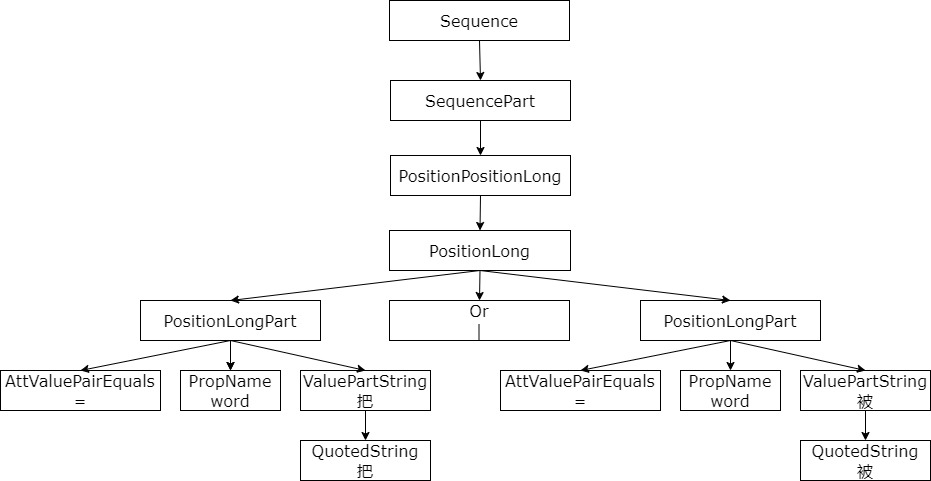
\includegraphics[width=0.7\textwidth]{image/yufashu.jpg}
	\caption{CQL语法树}
	\label{fig:yufashu}
\end{figure}

\subsection{倒排索引表设计}

检索和核心任务是完成检索词到文档的匹配,原始文本经过统一编码,段落分割、句子分割等预处理后,形成统一格式的语料数据。倒排索引工具,首先将传入的语料数据进行分段、分句操作,然后让每一句话通过分词工具进行分词以及标注词性,建立倒排索引表。

文档包含的信息是具有层次结构的,一篇文档,有很多属性信息包括:作者、文件名称、文件类型、文件大小、创建时间等信息,文件的内容还可以分为多个段落,每个段落由多个句子构成,在建立倒排索引时,根据语料库提供的范围约束条件,建立文档、段落、句子三级倒排索引结构。

用户输入的检索词不一定与语料库存储的词语一致,设计的倒排索引结构需要支持用户在文档中任意位置查询。比如在语料库中包含“和平共处”,被切分为“和平”、“共处”两个词语,但如果用户使用“和平共处”检索时,仍然希望能够匹配到这份语料。因此倒排索引除了能够通过词语找到对应语料之外,还需要支持范围检索能力,能够根据用户的输入,找到与该输入匹配的语料的能力。

建立词语倒排索引分为四个步骤,第一步将语料库中文档ID化,即文档进行分词与词性标注,将文档内容转换为词语ID序列。第二步将ID化后的文档,依次遍历每一个词语ID,并以这个词语ID作为子句起点,加入排序列表,由于这个过程会产生大量的子句,因此在排序的时候按照子句句首词语进行分组排序。第三步,排序后获得了文档范围内所有词语的排序位置,生成词语排序位置索引表,这个表的数据可以看作是一个有序子句列表,可以直接用来检索匹配。第四步,为了优化检索速度,使用有序子句列表生成词语匹配范围表,词语匹配范围表直接可以通过词语ID返回词语在有序字句表中匹配的起始位置和结束位置。

\begin{figure}[!h]
	\centering
	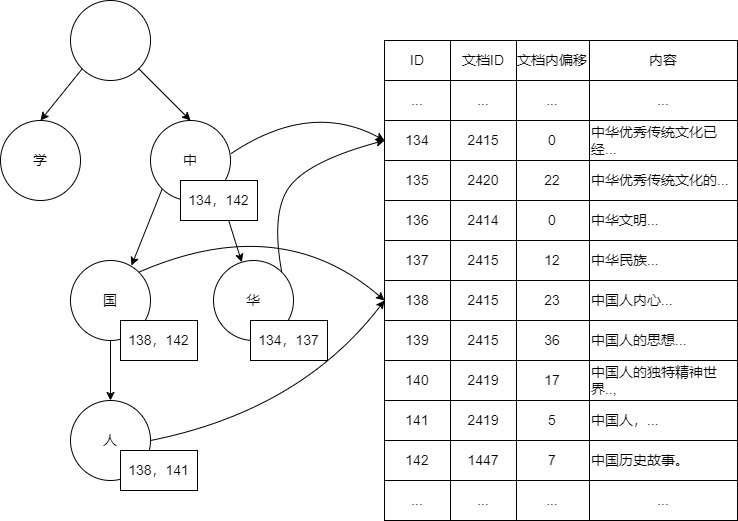
\includegraphics[width=0.8\textwidth]{image/daopaibiao.jpg}
	\caption{倒排索引表}
	\label{fig:daopaibiao}
\end{figure}

\subsection{检索表达式转换}

在语料库的查询操作中,一个核心步骤是将用户提供的CQL查询语句转换成能够被语料库系统识别和执行的语料库检索表达式。这个转换过程涉及到解析CQL语句,并构建出相应的语料库检索表达式的三个核心组成部分:查询语句、约束条件以及检索范围。

查询语句是构成检索表达式的基础元素,它们对应于CQL查询语句中的检索单元。这些查询语句是可以执行的具体查询指令,能够直接对语料库进行相关的数据检索。

条件约束在检索表达式中起着至关重要的作用。这些条件是由CQL查询语句中的检索条件转换而来的。约束条件确保了检索单元之间的关系符合用户的查询意图,它们对检索单元进行逻辑上的连接和限制,从而保证了检索结果的准确性和相关性。

范围约束则是由CQL中的检索范围所指定的。这个范围限定了检索单元语料库中同现位置的限制,用户可以指定时在句子范围、段落范围或者文档范围内进行数据匹配。

为了实现CQL到检索表达式的转换,系首先需要构建一棵CQL语法树,然后通过遍历这棵语法树,找到与CQL语句相对应的节点。这些节点包含了构建检索表达式所需的所有信息。接下来会将这些节点元素逐一转换为语料库查询表达式的对应元素,这一过程确保了CQL语句中的每一个查询条件都能被准确地转换成语料库检索表达式对应的内容。在完成转换后,系统就可以调用语料库的检索方法,执行具体的语料查询操作了。

\subsection{两阶段检索策略}

语料库检索不仅需要实现检索单元的精确匹配,还需验证各检索单元在语料中的位置和距离关系是否符合预设约束。在处理多段检索单元时,先筛选出符合匹配条件的句子,再进行约束条件的验证和筛选,可以显著提升检索效率。因此,本文提出一种两阶段检索策略。

在第一阶段,我们专注于检索单元的匹配。通过执行忽略位置和距离约束的检索表达式,从语料库中检索出所有可能的匹配语料。对于简单检索式,我们直接查询对应的倒排索引表,快速返回匹配结果。对于包含逻辑运算的复合检索式,我们通过语法解析构建检索树,然后遍历树并执行逻辑运算,以获得复合检索的结果。

在第二阶段,我们对第一阶段获取的语料进行更深入的筛选。具体而言,我们依据位置和距离约束条件,对上一阶段返回的匹配文档进行细致的评估。这些文档会根据检索语句中的具体约束条件,如词性约束等,返回相应的详细信息。在执行这一阶段的筛选时,我们从文档的开始位置,逐一核查检索单元的匹配位置是否符合预设的约束条件。由于单个文档内可能存在多个与检索单元相匹配的位置,我们采用动态规划算法,从起始检索单元开始,逐个检查其匹配位置是否满足过滤条件。只有当所有检索单元都完全符合要求时,我们才将该文档添加到最终的候选列表中。

此外,我们采用了一种高效的词语匹配策略:对于字典内的词语,直接返回其精确匹配的候选范围;若词语不在字典内,则返回该词语中最长连续子串所匹配的候选范围。随后,在该范围内通过二分查找算法进一步确定精确的匹配候选范围。以“和平共处”为例,当在词典树中从第一个字开始进行匹配时,匹配至“平”字后若无相应子节点可匹配,系统便会在“和平”这一最长匹配子串所对应的候选范围内,利用二分查找算法精确定位“和平共处”的候选范围。

值得注意的是,合并不同检索单元以及复合检索式内部的简单检索结果是一个技术挑战。传统的倒排索引表存储有序文档ID列表,便于通过跳表操作快速合并列表。然而,在我们的方法中,由于词语不是固定的索引单位,且对应的文档ID无序,因此无法采用传统的合并方式。为解决这个问题,我们设计了一个与文档数量相同的位数组,其中每位表示对应文档是否匹配。在合并两个检索表达式的结果时,只需执行逻辑运算,即可迅速完成合并操作。这种方法显著提高了检索效率,并优化了检索过程的性能。

%具体流程如算法~\ref{alg:getmatchdocflags}所示。
%\begin{algorithm}[H]
%	\caption{Get the query matching document ID flags}
%	\label{alg:getmatchdocflags}
%	\SetKwInput{KwInput}{$querys = \left\{ q_1, q_2, \ldots, q_n \right\}$}
%	\SetKwInput{KwOutput}{$document\ id\ list$}
%	\DontPrintSemicolon
%	
%	\KwInput{Input}
%	\KwOutput{Output}
%		
%	% Set Function Names
%	\SetKwFunction{FSum}{GetMatchDocFlags}
%	
%	% Write Function with word ``Def''
%	\SetKwProg{Fn}{Def}{:}{}
%	\Fn{\FSum{$query$}}{
%		op = query.op\;
%		\uIf {op = 'AND'} {
%			flags1 $\leftarrow$ GetMatchDocFlags(query.first)\;
%			flags2 $\leftarrow$ GetMatchDocFlags(query.second)\;
%			flags $\leftarrow$ flag1 \& flags2\;
%		}\uElseIf {op = 'OR'} {
%			flags1 $\leftarrow$ GetMatchDocFlags(query.first)\;
%			flags2 $\leftarrow$ GetMatchDocFlags(query.second)\;
%			flags $\leftarrow$ flag1 \textbar \ flags2\;
%		} \uElse {
%			flags $\leftarrow$ SearchCorpus(query.data)\;
%		}
%		
%		\KwRet flags\;
%	}
%	\;
%flags $\leftarrow$ DefaultMatchFlags()\;
%\ForEach{$q_i \in querys$}{
%	flags $\leftarrow$ flags \& GetMatchDocFlags($q_i$)
%}
%	
%	\KwRet flags\;
%\end{algorithm}


\section{实验}

本研究利用《人民日报》文本语料,建立了语料数据库,采用BlackLab与自研查询引擎进行检索词检出以及检索效率对比实验。比较了CCL和CQL两种检索语言。

\subsection{数据集}

实验采用的数据集为《人民日报》图文数据库2005年-2015年的文本语料。对语料使用斯坦福分词工具标记生成collun格式数据文件,分别使用BlackLab与本文编写的语料库查询引擎建立索引,生成语料数据库。并根据语料编写COL语句,用于召回率测试和性能测试。

\subsection{检索词实验}

随机选取人民日报的若干句子,采用人工抽取检索词的方式、以及通过分词工具自动分词,使用分词结果进行语料库查询测试。可以看到有24.2\% 的人工抽取的检索词无法检出结果,分词工具的分词数据中有17.5\%使用BlackLab无法检索出结果,而通过本文的检索工具能够全部检出。 

\subsection{检索速度实验}

人工构造了典型的CQL检索式,与BlackLab进行检索速度对比试验,每条语句执行10次,取响应时间的平均值(单位:毫秒)。具体数值如表所示。

\begin{table}[h]
	\begin{center}
		\begin{tabular}{c|c|c}
			\hline \bf CCL检索式 & \bf BlackLab & \bf 本文 \\ \hline
			[word=“的”][] \{ 0, 10 \} [word='的'] & 11 & 12.4 \\ \hline
			[word = '文化'][]\{0,2\}[word = '交流'] & 1921 & 9.5 \\
			\hline
			[word='把'][]\{1,1\}[word='给'] & 24 & 8.7 \\
			\hline
			[word = '与其'][word = '不如'] & 34 & 4.9 \\
			\hline
			[word='把'  \textbar word='被'][]\{2,4\}[word='给'] & 1004 & 43.4 \\
			\hline
			[word = '爱'][pos='v'][word = '不'][pos='v'] & 12 & 8.3 \\
			\hline
			[word = '宁可'][]\{\}[word = '也'] & 137 & 6.4 \\
			\hline
			[word = '澡'][ word = '洗'] & 19 & 5.3 \\
			\hline
			[word = '一边'][]\{3,3\}[word = '一边'] & 131 & 7.4 \\
			\hline
		\end{tabular}
	\end{center}
	\caption{\label{speed-table} 查询速度对比}
\end{table}

通过数据对比,可以看到设计的检索引擎的检索速度优于BlackLab,平均检索速度快40\%(110.9/182) 。

\subsection{检索式对比}

CCL语料库检索式设计十分完善。然而,对于初学者而言,其学习成本相对较高。具体而言,CCL查询表达式中定义了多达13个特殊符号,其检索式由基本项、简单项、复杂项、过滤项、子句等多个部分组成,这就要求使用者必须掌握这些基础知识才能有效地编写检索表达式。

相比之下,CQL语言在语法上显得更为简洁直观。通过使用CQL表达式,用户能够更快速地掌握语料库的使用方法,无需投入过多的时间和精力去学习和记忆复杂的符号和规则。通过对比一些常用的检索式写法,我们可以清晰地看到CQL的简洁性。相较于CCL中使用的特殊符号和复杂的结构,CQL提供了一种更为直接和自然的方式来表达检索需求,从而提高了检索的效率和用户体验。

\begin{table}[h]
	\begin{center}
		\begin{tabular}{c|c}
			\hline \bf CCL检索式 & \bf CQL检索式 \\ \hline
			计算机硬件 & [word='计算机硬件'] \\ \hline
			把 \textbar 被 & [word='把' \textbar word='被'] \\ \hline
			被+1把\$6给 & [word='被'][]\{1\}[word='把']\{0,6\}[word='给'] \\ \hline
			与其\$[2-4]不如 & [word = '与其'][]\{2,4\}[word = '不如'] \\ \hline
		\end{tabular}
	\end{center}
	\caption{\label{ccl-table} CQL与CCL检索式对比}
\end{table}

通过对比可以看到,CCL检索式和CQL检索式能够实现的功能基本相同,但CQL检索式的形式和规则比较简单,采用统一的约束符号,更容易被掌握。

CCL的表达式,更为简洁,例如:查找同时含有“能力”和“大”的句子,且“能力”和“大”之间的间隔在3个字之内,二者的先后次序不受限制。使用CCL检索式编写:“能力\#3大” 能够实现这个功能,用CQL编写表达式为,A:[ word=“能力” \textbar word='大'][]\{3,3\}B:[word='能力' \textbar word='大']::A!=B,较CCL繁琐很多。

尽管CCL功能完善,但其复杂的符号和结构增加了学习难度。相比之下,CQL语法简洁直观,更易于表达检索需求,提高了检索效率和用户体验。


%a&b
%
%a1a2
%分开也能检出
%

100例子,分词工具



\section{结论}

本文对语料库检索进行深入探索,采用CQL作为语言库检索语言,通过ANTLR工具将CQL语言解析问语法树,设计和构建了C++版本的语料库检索引擎,优化了倒排索引表中词语检索匹配策略,可以有效仅实现非词表词语,以及词语前缀的匹配。采用二阶段检索策略,以及候选标记位过滤方案,提升语料库的检索速度实现表明本文设计的检索引擎高效准确。

综上所述,本研究验证了自研查询引擎在检索覆盖率和速度方面的优势,并展示了CQL的简洁性和直观性,为语料库检索技术的研究和应用提供了有益参考和高效工具。

% include your own bib file like this:
\bibliographystyle{ccl}
\bibliography{ccl2024-zh}

\end{CJK*}
\end{document}

